\whiteBGstarBegin
\setcounter{section}{0}

\section{Tự luận}
\begin{enumerate}[label=\bfseries Câu \arabic*:]
			\item \mkstar{3}
		
		\cauhoi{Một ô tô A chạy đều trên một đường thẳng với vận tốc $\SI{40}{km/h}$. Một ô tô B đuổi theo ô tô A với vận tốc $\SI{60}{km/h}$. Xác định vận tốc của ô tô B đối với ô tô A và của ô tô A đối với ô tô B.}
		\loigiai{
			Chọn chiều dương là chiều chuyển động của hai xe.
			
			$\overrightarrow{v_\text{AD}}$ là vận tốc của xe A đối với đất;
			
			$\overrightarrow{v_\text{BD}}$ là vận tốc của xe B đối với đất;
			
			$\overrightarrow{v_\text{BA}}$ là vận tốc của xe B đối với xe A.
			
			Theo công thức cộng vận tốc:
			$$\overrightarrow{v_\text{AB}} = \overrightarrow{v_\text{AD}}+\overrightarrow{v_\text{DB}} \Rightarrow \overrightarrow{v_\text{AB}} = \overrightarrow{v_\text{AD}} - \overrightarrow{v_\text{BD}}$$
			
			Do hai xe chuyển động ngược chiều nên
			$$v_\text{AB} = 40-60=-20\ \text{km/h}$$
			
			Vậy $v_\text{BA} = 20\ \text{km/h}$.
		}
		\item \mkstar{3}
		
		\cauhoi
		{A ngồi trên một toa tàu chuyển động với vận tốc $\SI{15}{km/h}$ đang rời ga. B ngồi trên một toa tàu khác đang chuyển động với vận tốc $\SI{10}{km/h}$ đang đi ngược chiều vào ga. Hai đường tàu song song với nhau. Tính vận tốc của B đối với A.
		}
		\loigiai
		{Chọn chiều dương là chiều chuyển động của tàu A.
			
			$\overrightarrow{v_\text{AD}}$ là vận tốc của tàu A đối với đất;
			
			$\overrightarrow{v_\text{BD}}$ là vận tốc của tàu B đối với đất;
			
			$\overrightarrow{v_\text{BA}}$ là vận tốc của tàu B đối với tàu A.
			
			Theo công thức cộng vận tốc:
			$$\overrightarrow{v_\text{BD}} = \overrightarrow{v_\text{BA}}+\overrightarrow{v_\text{AD}} \Rightarrow \overrightarrow{v_\text{BA}} = \overrightarrow{v_\text{BD}} - \overrightarrow{v_\text{AD}}=\overrightarrow{v_\text{BD}} + \overrightarrow{-v_\text{AD}}$$
			
			Do A và B chuyển động ngược chiều nên
			$$v_\text{AB} = v_\text{BD} + v_\text{DA} = -10-15 = \SI{-25}{km/h}$$
			
			Vận tốc của tàu B đối với tàu A có độ lớn $\SI{25}{km/h}$ và ngược chiều so với chiều chuyển động của tàu A.
		}
		\item \mkstar{3}
	
	\cauhoi
	{
		Hai người đi xe đạp từ A đến C, người thứ nhất đi theo đường từ A đến B, rồi từ B đến C; người thứ hai đi thẳng từ A đến C. Cả hai đều về đích cùng một lúc. Hãy tính quãng đường đi được và độ dịch chuyển của người thứ nhất và người thứ hai. So sáng và nhận xét kết quả.
		
		\begin{center}
			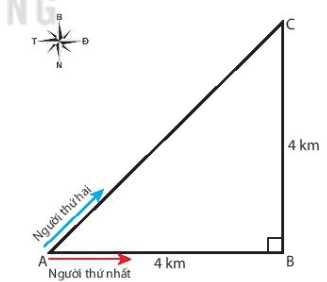
\includegraphics[scale=1]{../figs/VN10-2022-PH-TP004-5.jpg}
		\end{center}
	}
	
	\loigiai
	{	
		
		Quãng đường đi được của người thứ nhất:
		
		$$s_1 = \text{AB} + \text{BC} = 4+4 = \SI{8}{km}.$$
		
		Vì ABC là tam giác vuông nên độ lớn của độ dịch chuyển $\vec{\text{AC}}$ của người thứ nhất được tính bằng công thức:
		
		$$d_1 = \sqrt{\text{AB}^2 + \text{BC}^2} \approx \SI{5,7}{km}.$$
		
		Vì ABC là tam giác vuông cân nên góc CAB bằng $45^\circ$. Hướng của độ dịch chuyển là hướng $45^\circ$ Đông - Bắc. Độ dịch chuyển của người thứ nhất là $d_1 = \SI{5,7}{km}$ (hướng $45^\circ$ Đông - Bắc).
		
		Quãng đường đi được của người thứ hai là:
		
		$$s_2 = \text{AC} = \SI{5,7}{km}.$$
		
		Độ dịch chuyển của người thứ hai là:
		
		$$d_2 = \SI{5,7}{km}$$
		
		và hướng $45^\circ$ Đông - Bắc.
	}
	
	\item \mkstar{3}
	
	\cauhoi
	{   
		Trên đoàn tàu đang chạy thẳng với vận tốc trung bình $\SI{36}{km/h}$ so với mặt đường. Hãy xác định vận tốc của hành khách đối với mặt đường nếu người này chuyển động về cuối đoàn tàu với vận tốc có cùng độ lớn $\SI{1}{m/s}$.
	}
	\loigiai
	{
		
		Đổi: $\SI{36}{km/h} = \SI{10}{m/s}$.
		
		Gọi:
		
		$\vec v_{1,2}$ là vận tốc của hành khách so với tàu.
		
		$\vec v_{2,3}$ là vận tốc của tàu so với mặt đường.
		
		$\vec v_{1,3}$ là vận tốc của hành khách so với mặt đường.
		
		Ta có:
		
		$$\vec v_{1,3} = \vec v_{1,2} + \vec v_{2,3}.$$
		
		Do hành khách chuyển động về cuối đoàn tàu, tức là ngược chiều chuyển động của đoàn tàu nên ta có:
		
		$$v_{1,3} = - v_{1,2} + v_{2,3} = \SI{9}{m/s}.$$
	
		
	}
	\item \mkstar{3}
	
	\cauhoi
	{
		Một người bơi trong bể bơi yên lặng có thể đạt tới vận tốc $\SI{1}{m/s}$. Nếu người này bơi xuôi dòng sông có dòng chảy với vận tốc $\SI{1}{m/s}$ thì có thể đạt vận tốc tối đa là bao nhiêu?
	}
	\loigiai
	{
		Gọi:
		
		$\vec v_{1,2}$ là vận tốc của người so với nước.
		
		$\vec v_{2,3}$ là vận tốc của nước so với bờ.
		
		$\vec v_{1,3}$ là vận tốc của người so với bờ.
		
		Ta có:
		
		$$\vec v_{1,3} = \vec v_{1,2} + \vec v_{2,3}.$$
		
		- Khi người bơi trong bể nước yên lặng, thì $v_{2,3} = 0$:
		
		$$v_{1,2} = v_{1,3} = \SI{1}{m/s}.$$
		
		- Khi người này bơi xuôi dòng chảy với vận tốc $v_{2,3} = \SI{1}{m/s}$:
		
		
		$$v_{1,3} = v_{1,2} + v_{2,3} = \SI{2}{m/s}.$$
		
		Vậy nếu người này bơi xuôi dòng sông có dòng chảy với vận tốc $\SI{1}{m/s}$ thì có thể đạt vận tốc tối đa là $\SI{2}{m/s}.$
		
	
	}
	\item \mkstar{3}
	
	\cauhoi
	{
		Một ca nô chạy hết tốc lực trên mặt nước yên lặng có thể đạt $\SI{21,5}{km/h}$. Ca nô này chạy xuôi dòng sông trong 1 giờ rồi quay lại thì phải mất 2 giờ nữa mới về tới vị trí ban đầu. Hãy tính vận tốc chảy của dòng sông.
	}
	\loigiai
	{
		Gọi:
		
		$\vec v_{1,2}$ là vận tốc của canô so với nước.
	
		
		$\vec v_{2,3}$ là vận tốc của nước so với bờ.
		
		
		$\vec v_{1,3}$ là vận tốc của canô so với bờ.
		
		Ta có:
		
		$$\vec v_{1,3} = \vec v_{1,2} + \vec v_{2,3}.$$
		
		- Khi canô chạy trên mặt nước yên lặng, tức $v_{2,3} = 0$:
		
		
		$$v_{1,2} = v_{1,3} = \SI{21,5}{km/h}.$$
		
		- Khi canô chạy xuôi dòng sông, ta có:
		
		$$v_{1,3} = v_{1,2} + v_{2,3} \Rightarrow t_1 = \dfrac{d}{v_{1,2} + v_{2,3}}\ (1).$$
		
		- Khi canô quay lại, ta có:
		
		$$v'_{1,3} = v_{1,2} - v_{2,3} \Rightarrow t_2 = \dfrac{d}{v_{1,2} - v_{2,3}}\ (2).$$
	
		Thay các đại lượng của đề vào (1) và (2) ta suy ra:
		
		$$\begin{cases}
			d = \SI{28,67}{km}.\\
			v_{2,3} = \SI{7,17}{km/h}.
		\end{cases}$$
	
		Vậy vận tốc chảy của dòng sông là $\SI{7,17}{km/h}$.
		
		
	}
	\item \mkstar{3}
	
	\cauhoi
	{
		Một ca nô chạy trong hồ nước yên lặng có vận tốc tối đa $\SI{18}{km/h}$. Nếu ca nô chạy ngang một con sông có dòng chảy theo hướng Bắc - Nam với vận tốc lên tới $\SI{5}{m/s}$ thì vận tốc tối đa nó có thể đạt được so với bờ sông là bao nhiêu và theo hướng nào?
	}
	\loigiai
	{
		\begin{center}
			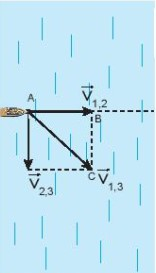
\includegraphics[scale=1]{../figs/VN10-2022-PH-TP005-4.jpg}
		\end{center}
		Gọi vận tốc của ca nô đối với mặt nước là $\vec v_{1,2}$; 
		
		Vận tốc của nước chảy đối với bờ sông là $\vec v_{2,3}$. 
		
		Vận tốc của ca nô đối với bờ sông:
		
		$$\vec v_{1,3} = \vec v_{1,2} + \vec v_{2,3}.$$
		
		Suy ra:
		
		$$v_{1,3} = \sqrt{ v_{1,2}^2 + v_{2,3}^2} = \SI{7,07}{m/s}.$$
		
		Vì $\text{AB} = \text{BC}$ nên tam giác ABC là tam giác vuông cân và góc A bằng $45^\circ$. Hướng của vận tốc nghiêng $45^\circ$ theo hướng Đông - Nam.
	}
	\item \mkstar{3}
	
	\cauhoi
	{
		Một máy bay đang bay theo hướng Bắc với vận tốc $\SI{200}{m/s}$ thì bị gió từ hướng Tây thổi vào với vận tốc $\SI{20}{m/s}$. Xác định vận tốc tổng hợp của máy bay lúc này.
	}
	\loigiai
	{
		Gọi:
		
		$\vec v_{1,2}$ là vận tốc của máy bay so với gió.
		
		$\vec v_{2,3}$ là vận tốc của gió so với đường bay.

		$\vec v_{1,3}$ là vận tốc của máy bay so với đường bay.
		
		Ta có:
		
		$$\vec v_{1,3} = \vec v_{1,2} + \vec v_{2,3}.$$
		
		Vận tốc tổng hợp của máy bay lúc này là
		
		$$v_{1,3} = \sqrt{v_{1,2}^2 + v^2_{2,3}} = \SI{201}{m/s}.$$
	}
		\item \mkstar{4}
	
	\cauhoi
	{
		Trên đoàn tàu đang chạy thẳng với vận tốc trung bình $\SI{36}{km/h}$ so với mặt đường, một hành khách đi về đầu tàu với vận tốc $\SI{1}{m/s}$ so với mặt sàn tàu.
		\begin{center}
			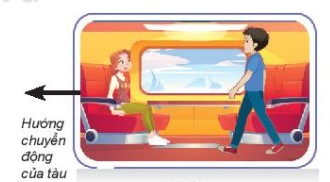
\includegraphics[scale=1]{../figs/VN10-2022-PH-TP005-3.jpg}
		\end{center}
		\begin{enumerate}[label=\alph*)]
			\item Hành khách này tham gia mấy chuyển động?
			\item Làm cách nào để xác định được vận tốc của hành khách đối với mặt đường.
		\end{enumerate}
	}
	\loigiai
	{
		\begin{enumerate}[label=\alph*)]
			\item Hành khách này tham gia 2 chuyển động: Chuyển động với vận tốc $\SI{1}{m/s}$ so với sàn tàu và chuyển động do tàu kéo đi với vận tốc bằng vận tốc của tàu so với mặt đường. Chuyển động của hành khách so với mặt đường là tổng hợp của hai chuyển động trên.
			\item Gọi:
			
			- $\vec v_{1,2}$ là vận tốc của hành khách so với tàu.
			
			- $\vec v_{2,3}$ là vận tốc của tàu so với mặt đường.
			
			- $\vec v_{1,3}$ là vận tốc của hành khách so với mặt đường.
			
			Thì:
			
			$$\vec v_{1,3} = \vec v_{1,2} + \vec v_{2,3}$$
			
			Vì các chuyển động trên đều là chuyển động thẳng theo hướng chạy của đoàn tàu nên:
			
			$$v_{1,3} = v_{1,2} + v_{2,3} = \SI{11}{m/s}.$$
			
			Hướng của vận tốc là hướng đoàn tàu chạy.
		\end{enumerate}
	}
	
		\item \mkstar{3}
	
	\cauhoi
	{
		Một người bơi ngang từ bờ bên này sang bờ bên kia của một dòng sông rộng $\SI{50}{m}$ có dòng chảy theo hướng từ Bắc xuống Nam. Do nước sông chảy mạnh nên khi sang đến bờ bên kia thì người đó đã trôi xuôi theo dòng nước $\SI{50}{m}$. Xác định độ dịch chuyển của người đó.
	}
	
	\loigiai
	{
		\begin{center}
			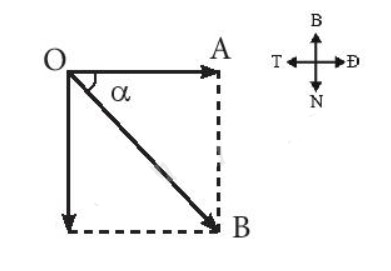
\includegraphics[scale=0.6]{../figs/VN10-2022-PH-TP0001-2.jpg}
		\end{center}
		Người bơi ngang từ bờ bên này sang bên kia theo dự định là OA = $\SI{50}{m}$.
		
		Thực tế, do nước sông chảy mạnh nên vị trí của người đó ở vị trí B, ta có AB = $\SI{50}{m}$.
		
		$\Rightarrow$ Độ dịch chuyển:
		
		$$\Rightarrow\text{OB} = \sqrt{\text{OA}^2 + \text{AB}^2} = \SI{70,7}{km}.$$ 
	}

\end{enumerate}